\chapter{Metodologia}\label{cap:metodologia}

\section{Visão geral}

O estudo é organizado como uma cadeia de reconstrução e estruturação. O estágio neural é executado com DM-NeRF sobre DM-SR. A partir do modelo treinado, são produzidas métricas de teste e uma malha triangular com identificadores de instância por vértice. O pós-processamento transforma essa saída em objetos independentes, seleciona um candidato geométrico a piso, regulariza essa superfície quando a seleção é válida e exporta uma cena em SDFormat.

A Figura~\ref{fig:method_pipeline} apresenta a sequência completa e indica a medida associada a cada transformação. Essa correspondência entre etapa e medida orienta o protocolo experimental e impede que qualidade visual seja tomada como substituta da qualidade geométrica ou funcional.

\begin{figure}[H]
  \centering
  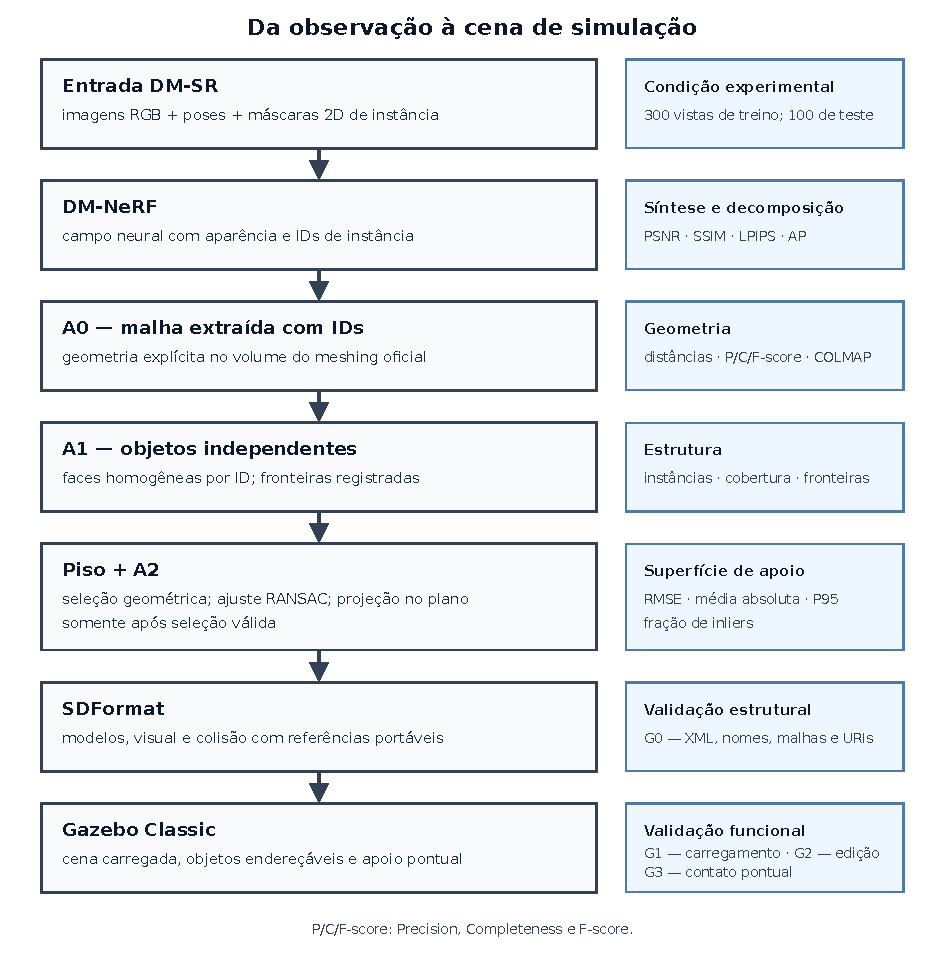
\includegraphics[width=0.90\textwidth]{method_pipeline.pdf}
  \caption{Cadeia metodológica entre as observações do DM-SR e a cena no Gazebo Classic, com as medidas empregadas em cada etapa.}
  \label{fig:method_pipeline}
\end{figure}

Por convenção deste experimento, as condições da ablação interna são identificadas pelo prefixo A: A0 corresponde à malha extraída, A1 acrescenta a separação dos objetos e A2 acrescenta a regularização do piso. As verificações no Gazebo recebem o prefixo G e avançam da validação estática, G0, aos ensaios funcionais G1--G3. A numeração expressa, portanto, a progressão cumulativa da cadeia, e não uma nomenclatura própria do DM-NeRF.

As etapas e suas medidas são apresentadas na Tabela~\ref{tab:etapas}. A organização evita atribuir a uma etapa uma métrica que ela não pode alterar. A separação estrutural A1, por exemplo, não modifica intencionalmente as coordenadas das faces preservadas e, portanto, não é avaliada por PSNR ou por ganho de distância de superfície.

\begin{table}[H]
\centering
\small
\caption{Etapas da cadeia e medidas utilizadas.}
\label{tab:etapas}
\begin{tabularx}{\textwidth}{p{2.1cm}Y Y}
\toprule
\textbf{Etapa} & \textbf{Transformação} & \textbf{Medida principal} \\
\midrule
Neural & treinamento e avaliação do DM-NeRF & PSNR, SSIM, LPIPS e AP em vistas de teste \\
A0 -- malha & extração da malha & distâncias de superfície, Precision, Completeness e F-score \\
A1 -- objetos & separação por IDs explícitos & número de instâncias, cobertura de faces e fronteiras \\
A2 -- piso & regularização do candidato a piso & resíduos ao plano antes/depois \\
Gazebo & exportação e execução & verificações G0--G3 \\
\bottomrule
\end{tabularx}
\end{table}

\section{Conjunto de dados DM-SR}

O conjunto DM-SR fornece imagens RGB, poses de câmera, mapas bidimensionais de instância e uma malha tridimensional de referência. Para a cena \textit{study}, o experimento utiliza 300 imagens de treinamento e 100 vistas de teste do protocolo original. A malha de referência e os metadados de câmera são mantidos nas avaliações geométricas; quatro vistas de teste são usadas nas comparações qualitativas.

Quatro vistas reais da cena, extraídas do conjunto de teste, são apresentadas posteriormente junto às renderizações correspondentes do DM-NeRF (Figura~\ref{fig:render_comparison}). Essa comparação introduz visualmente a configuração doméstica/escritório e evita repetir as mesmas imagens em figuras distintas.

A malha de referência tem 437.008 vértices e 844.701 faces. O procedimento oficial de extração de malha do DM-NeRF utiliza o \textit{oriented bounding box} dessa referência para definir o volume e a orientação da consulta ao campo neural. Dessa forma, a referência participa da definição do domínio de extração, e as métricas geométricas são interpretadas dentro desse domínio.

Os mapas de instância do DM-SR utilizam identificadores inteiros, mas os artefatos inspecionados não fornecem um catálogo semântico completo que associe cada ID a uma classe do ambiente. Em particular, não foi encontrada uma associação oficial entre um ID e a classe piso.

\section{Treinamento e avaliação do DM-NeRF}

A reprodução utiliza a implementação oficial do DM-NeRF. A configuração final usa 64 amostras no passe inicial, 128 amostras adicionais, 3.072 raios no treinamento e 1.024 raios no avaliador. O treinamento foi realizado com precisão mista automática; a avaliação final e a extração da malha foram mantidas em FP32.

O avaliador oficial calcula a razão sinal-ruído de pico (PSNR), o índice de similaridade estrutural (SSIM) \citep{wang2004ssim} e a distância perceptual LPIPS \citep{zhang2018lpips} para síntese de vistas; o PSNR segue a definição usada no protocolo do DM-NeRF \citep{wang2023dmnerf}. Para decomposição, a interseção sobre união (IoU) mede a sobreposição entre uma máscara predita e sua referência, e a precisão média (AP) resume a qualidade das detecções em um limiar de IoU, conforme o avaliador do método. Valores maiores indicam melhor correspondência. São usados os limiares de IoU 0,50, 0,75, 0,80, 0,85, 0,90 e 0,95. A função de perda e as métricas emitidas durante o treinamento não são utilizadas como resultados de teste.

\section{Extração da malha e contrato de rótulos}

Após o treinamento, o campo neural é consultado no volume definido pelo procedimento oficial e convertido em malha triangular. A condição A0 reúne a geometria extraída e um vetor de identificadores de instância associado aos vértices. As cores presentes na visualização são usadas somente para apresentação; a separação estrutural consulta os identificadores explícitos, e não valores RGB.

Antes de separar objetos, o contrato verifica a quantidade e a ordem dos vértices, os índices dos triângulos, a topologia e a finitude das coordenadas. Essa verificação impede a associação de IDs a uma malha com ordem de vértices diferente. A malha final contém 356.272 vértices e 710.928 faces.

\section{Separação estrutural (A1)}

A condição A1 é formada a partir de A0. Para cada triângulo, são consultados os IDs de seus três vértices. Uma face é atribuída a uma instância somente quando os três IDs coincidem. Faces com IDs diferentes são classificadas como faces de fronteira e permanecem fora das malhas individuais. A decisão evita escolher arbitrariamente um dos rótulos presentes na face.

Para cada instância com faces homogêneas, os vértices utilizados são remapeados e uma malha independente é exportada. São registrados o ID, o número de vértices e faces, a área, os limites espaciais e o centroide. A cobertura de faces homogêneas e a quantidade de fronteiras são calculadas sobre a topologia original.

\section{Seleção geométrica do piso}

Como não há rótulo semântico oficial para o piso, a seleção usa uma heurística geométrica definida antes da observação da malha final. Cada instância é analisada somente pelas faces homogêneas. O plano principal é obtido por covariância dos vértices dessas faces com ponderação pela área dos triângulos. São calculados área, fração de área aproximadamente horizontal, normal, altura e RMSE do ajuste.

Uma instância é elegível quando satisfaz simultaneamente: área de pelo menos 0,5 m$^2$; pelo menos 85\% da área com orientação de até 15 graus da vertical; normal do plano dentro do mesmo limite angular; RMSE de no máximo 0,03 m; e posição na faixa inferior da cena, definida pelo percentil 1 das alturas acrescido de 20\% da amplitude vertical. O eixo vertical da malha é +Y.

Entre candidatas elegíveis, a maior área é escolhida se a segunda candidata tiver área inferior a 80\% da primeira. Caso contrário, a saída é ambígua. Se nenhuma instância for elegível, a saída é ``não identificada''. Em ambos os casos de abstenção, A2 é bloqueada. A regra não utiliza cor, número de ID ou associação histórica como critério semântico.

\section{Regularização do piso (A2)}

Quando existe candidato válido, os vértices associados ao ID selecionado são usados no algoritmo \textit{Random Sample Consensus} (RANSAC) de \citet{fischler1981ransac}, que ajusta um modelo robusto mesmo na presença de pontos discrepantes. O limiar é 2 cm e a semente é fixa. O plano final é ajustado aos inliers. A regularização projeta apenas os vértices da instância selecionada sobre esse plano. A topologia e os IDs não são alterados.

O efeito é medido sobre o mesmo subconjunto antes e depois da projeção. São reportados erro absoluto médio, RMSE, P95 e fração de inliers. Uma redução desses resíduos indica apenas maior aderência ao plano estimado. Como a operação é uma projeção, a redução é esperada por construção e não demonstra aumento de fidelidade global em relação ao ambiente real.

\section{Exportação para Gazebo Classic}

A exportação gera mundos SDFormat com referências relativas. A0 é representada por uma malha única. A1 e A2 são representadas por modelos independentes derivados das instâncias. Cada modelo possui um link, um elemento visual e um elemento de colisão apontando para a mesma malha triangular. O referencial +Y da reconstrução é rotacionado para +Z do Gazebo por uma transformação rígida comum.

A validação G0 verifica XML, nomes únicos, existência das malhas, caminhos relativos, escalas positivas e correspondência entre visual e colisão. Essa etapa não executa a física e não substitui o parser nativo do Gazebo. G1, G2 e G3 verificam, respectivamente, carregamento real, manipulação independente e suporte/colisão do piso.
